\documentclass[12pt]{article}

\usepackage{hyperref}
\usepackage{algorithm}
\usepackage[noend]{algpseudocode}
\usepackage{tikz}
\usetikzlibrary{arrows.meta,arrows}

\begin{document}

\title{Inference of chemical compound types \\ using graph of chemical reactions}
\author{Yurii Lahodiuk \\ yura.lagodiuk@gmail.com}
\date{}
\maketitle

\begin{abstract}
% TODO: refactor
In this article we will consider representation of information about chemical interactions - from the point of view of graph theory. We will expose some properties of chemical reactions graph in order to infer types of chemical compounds, and do this in polynomial time. And, finally, I would like to provide detailed description of developed programming framework\cite{project_on_github} for approximate inference over pairwise Markov Random Fields, with appliance to solving of such problems as: decoding of Low-density parity-check codes, Coloring of graph, Fraud detection using network effects\cite{fraud_detection}.
\end{abstract}

\section{Problem statement}
Lets imagine simplified universe, where exists only few different \emph{types of chemical compounds}. 
%TODO: enumerate types of chemical compounds.
% E.g.: Water, Base, Acid, Salt, Acidic Salt, Acidic Oxide, Basic Oxide
Also there exists restrictions on \lq \lq allowed\rq \rq\ interactions between different compounds (lets call these restrictions -- \emph{types of chemical reactions}).
%TODO: enumerate types of chemical reactions.
% E.g.: Base + Acid --> Salt + Water, Acidic Oxide + Base --> Salt + Water, etc.
So, this is the only prior knowledge about our simplified universe\footnote{Of course, from the point of view of Chemistry Science - provided model of universe is very rough and strict. But, on the other hand - our model is pretty generic, because it does not depend on details of internal structure of compounds, or any other physical-chemistry factors: \emph{all prior knowledge we have - is just possible types of compounds, and axioms about allowed types of interaction}.}.\\

Now, imagine that we observed reactions of exact chemical compounds.
% TODO: enumerate examples of observed chemical reactions.
% E.g.: NaOH + H2SO4 --> Na2SO4 + H2O, Na2O + SO3 --> Na2SO4, etc.
So, the problem is: \textsl{having described prior knowledge about types of chemical compounds and restrictions on possible types of interactions - needed to \textbf{infer types of compounds, which participate in observed reactions}}. \\

In other words, we can formulate our problem - as \textsl{\textbf{finding of such configuration of types of compounds} from observed reactions, \textbf{which does not violate restrictions on allowed types of interaction}}.

\section{Na\"{\i}ve approach}
The most straightforward approach for solving of described problem -- would be just brute-force search of appropriate types for chemical compounds from observed reactions:

\begin{algorithm}
\caption{Brute-force search for appropriate types of compounds}\label{alg:brute_force}
\begin{algorithmic}[1]
\Procedure{AssignTypes}{$compoundTypeMap, compoundsList$}
    \If{\Call{Empty}{$compoundsList$}}
        \If{\Call{SolutionAcceptable}{$compoundTypeMap$}}
            \State \textbf{return $compoundTypeMap$}
        \EndIf
    \Else
        \State $compound \gets \Call{Head}{compoundsList}$
        \State $restCompounds \gets \Call{Tail}{compoundsList}$
        \For{$i \gets [1..\Call{Size}{PossibleCompoundTypes}]$}
            \State $type \gets PossibleCompoundTypes[i]$
            \State $compoundTypeMap[compound] \gets type$
            \State \Call{AssignTypes}{$compoundTypeMap,restCompounds$}
        \EndFor
    \EndIf
    %TODO: consider, whether it is fine to return sich message
    \State \textbf{return} \lq \lq Solution Does Not Exist\rq \rq
\EndProcedure
\\
\Procedure{SolutionAcceptable}{$compoundTypeMap$}
    \For{$i \gets [1..\Call{Size}{ObservedEquations}]$}
        \State $equation \gets ObservedEquations[i]$
        %TODO: consider better name than x
        %TODO: add comment to this function. E.g.: 
        % Input: "NaOH + H2SO4 --> Na2SO4 + H2O"
        % Output: "Base + Acid --> Salt + Water"
        \State $x \gets \Call{SubstituteTypes}{$equation, compoundTypeMap$}$
        \If{\Call{NotContains}{PossibleEquationTypes, x}}
            \State \textbf{return $false$}
        \EndIf
    \EndFor
    \State \textbf{return $true$}
\EndProcedure
\end{algorithmic}
\end{algorithm}

The problem of given approach, is such, that it leads to exponential complexity, with growth of number of observed compounds.

\section{Graph representation of observed reactions}

\centering{
% Might be helpful for the further refactoring: http://www.texample.net/tikz/examples/feature/nodes-and-shapes/
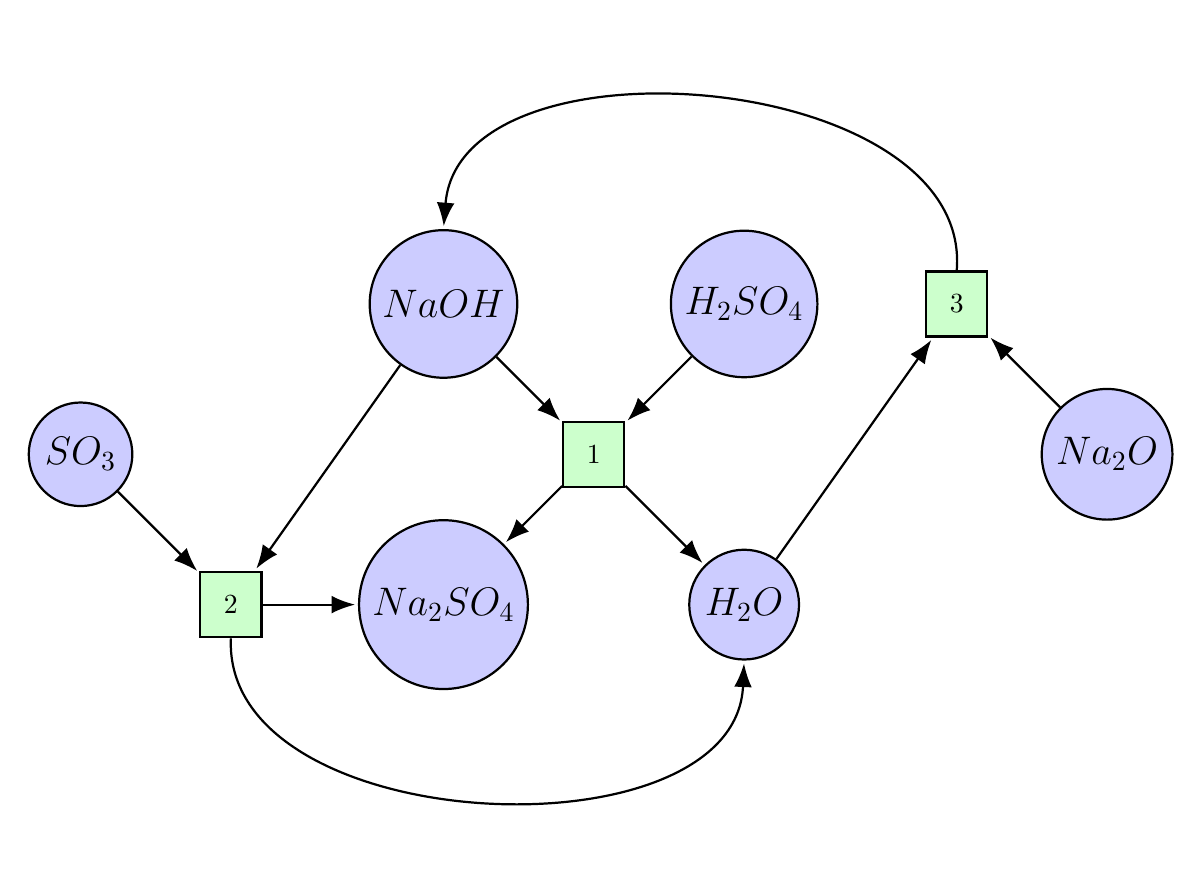
\begin{tikzpicture}[
    -{Latex[length=3mm]},
    shorten >=1pt,
    auto,
    node distance=2.7cm,
    thick,
    compound node/.style={circle,fill=blue!20,draw,font=\sffamily\Large\bfseries},
    reaction node/.style={draw,thick,fill=green!20,inner sep=.3cm}]

  \node[compound node] (NaOH) {$NaOH$};
  \node[reaction node] (Reaction1) [below right of=NaOH] {$1$};
  \node[compound node] (H2SO4) [above right of=Reaction1] {$H_{2}SO_{4}$};
  \node[compound node] (Na2SO4) [below left of=Reaction1] {$Na_{2}SO_{4}$};
  \node[compound node] (H2O) [below right of=Reaction1] {$H_{2}O$};  
  \node[reaction node] (Reaction2) [left of=Na2SO4] {$2$};  
  \node[compound node] (SO3) [above left of=Reaction2] {$SO_{3}$};  
  \node[reaction node] (Reaction3) [right of=H2SO4] {$3$};  
  \node[compound node] (Na2O) [below right of=Reaction3] {$Na_{2}O$};  

  \path[every node/.style={font=\sffamily\small}]
    (NaOH) 
         edge node[left] {} (Reaction1)
         edge node[right] {} (Reaction2)
    (H2SO4) 
         edge node[right] {} (Reaction1)
    (Reaction1) 
         edge node [right] {} (Na2SO4)
         edge node [left] {} (H2O)
    (SO3) 
         edge node [left] {} (Reaction2)
    (Reaction2) 
         edge node [left] {} (Na2SO4)
         edge [bend right = 90] node [right] {} (H2O)
    (H2O) 
         edge node [left] {} (Reaction3)
    (Na2O) 
         edge node [right] {} (Reaction3)
    (Reaction3) 
         edge [bend right = 90] node [right] {} (NaOH);
\end{tikzpicture}
}

\begin{thebibliography}{9}

\bibitem{project_on_github}
  \url{https://github.com/lagodiuk/java-loopy-belief-propagation}.

\bibitem{fraud_detection}
  Leman Akoglu, Rishi Chandy, Christos Faloutsos,
  \emph{Opinion Fraud Detection in Online Reviews by Network Effects}.

\bibitem{understanding_bp}
  Jonathan S. Yedidia, William T. Freeman, and Yair Weiss,
  \emph{Understanding Belief Propagation and its Generalizations},
  TR2001-22, 
  November 2001.

\end{thebibliography}

\end{document}